% Options for packages loaded elsewhere
\PassOptionsToPackage{unicode}{hyperref}
\PassOptionsToPackage{hyphens}{url}
\PassOptionsToPackage{dvipsnames,svgnames*,x11names*}{xcolor}
%
\documentclass[
  11pt,
]{article}
\usepackage{lmodern}
\usepackage{amssymb,amsmath}
\usepackage{ifxetex,ifluatex}
\ifnum 0\ifxetex 1\fi\ifluatex 1\fi=0 % if pdftex
  \usepackage[T1]{fontenc}
  \usepackage[utf8]{inputenc}
  \usepackage{textcomp} % provide euro and other symbols
\else % if luatex or xetex
  \usepackage{unicode-math}
  \defaultfontfeatures{Scale=MatchLowercase}
  \defaultfontfeatures[\rmfamily]{Ligatures=TeX,Scale=1}
\fi
% Use upquote if available, for straight quotes in verbatim environments
\IfFileExists{upquote.sty}{\usepackage{upquote}}{}
\IfFileExists{microtype.sty}{% use microtype if available
  \usepackage[]{microtype}
  \UseMicrotypeSet[protrusion]{basicmath} % disable protrusion for tt fonts
}{}
\makeatletter
\@ifundefined{KOMAClassName}{% if non-KOMA class
  \IfFileExists{parskip.sty}{%
    \usepackage{parskip}
  }{% else
    \setlength{\parindent}{0pt}
    \setlength{\parskip}{6pt plus 2pt minus 1pt}}
}{% if KOMA class
  \KOMAoptions{parskip=half}}
\makeatother
\usepackage{xcolor}
\IfFileExists{xurl.sty}{\usepackage{xurl}}{} % add URL line breaks if available
\IfFileExists{bookmark.sty}{\usepackage{bookmark}}{
\usepackage{hyperref}
}
\hypersetup{
  pdftitle={Corrigé du TP 8 Dichotomie - Newton},
  pdfauthor={Chenevois-Jouhet-Junier},
  colorlinks=true,
  linkcolor=Maroon,
  filecolor=Maroon,
  citecolor=Blue,
  urlcolor=Blue,
  pdfcreator={LaTeX via pandoc}}
\urlstyle{same} % disable monospaced font for URLs
\usepackage[top=20mm,left=20mm,right=20mm,heightrounded]{geometry}
\usepackage{listings}
\newcommand{\passthrough}[1]{#1}
\lstset{defaultdialect=[5.3]Lua}
\lstset{defaultdialect=[x86masm]Assembler}
\usepackage{graphicx}
\makeatletter
\def\maxwidth{\ifdim\Gin@nat@width>\linewidth\linewidth\else\Gin@nat@width\fi}
\def\maxheight{\ifdim\Gin@nat@height>\textheight\textheight\else\Gin@nat@height\fi}
\makeatother
% Scale images if necessary, so that they will not overflow the page
% margins by default, and it is still possible to overwrite the defaults
% using explicit options in \includegraphics[width, height, ...]{}
\setkeys{Gin}{width=\maxwidth,height=\maxheight,keepaspectratio}
% Set default figure placement to htbp
\makeatletter
\def\fps@figure{htbp}
\makeatother
\setlength{\emergencystretch}{3em} % prevent overfull lines
\providecommand{\tightlist}{%
  \setlength{\itemsep}{0pt}\setlength{\parskip}{0pt}}
\setcounter{secnumdepth}{5}

\title{Corrigé du TP 8 Dichotomie - Newton}
\author{Chenevois-Jouhet-Junier}
\date{}

%%%jolis boites

\usepackage{fancybox, graphicx}



%%%%%%%%%%%%%%%%Packages et Macros Frederic%%%%%%%%%%%%%%%%%%%%%%%%%%%%%


%%%%Insertion de liens hypertextes %%%%

            
%%%%%%%%%%PSTricks%%%%%%%%%%%%

\usepackage{pstricks,pst-plot,pst-text,pst-tree,pst-eps,pst-fill,pst-node,pst-math,pstricks-add,pst-xkey,pst-eucl}


%%%%%%%Tikz%%%%%%%%%%%%%%%
\usepackage{pgf,tikz,tkz-tab}
% Pour les tableaux de signes ou de variations avec tkz-tab voir https://zestedesavoir.com/tutoriels/439/des-tableaux-de-variations-et-de-signes-avec-latex/#1-13389_tikz-un-package-qui-en-a-dans-le-ventre
\usetikzlibrary{arrows}
\usetikzlibrary{shapes.geometric}
\usetikzlibrary{shapes.geometric}
\usetikzlibrary{petri}
\usetikzlibrary{decorations}
\usetikzlibrary{arrows}
\usetikzlibrary{math}
 %Variables must be declared in a tikzmath environment but
       % can be used outside
%       \tikzmath{int \n; \n = 508; \x1 = 1; \y1 =1; 
%                   %computations are also possible
%                    \x2 = \x1 + 1; \y2 =\y1 +3; } 


%%%%%%%%%%%%%%%%%%%%%%%%%%%%%%%%%%%%%%%%
%%%%%%%%%%%Commandes Tikz Perso%%%%%%%%%%%%%%%

% Définition des nouvelles options xmin, xmax, ymin, ymax
% Valeurs par défaut : -3, 3, -3, 3
\tikzset{
xmin/.store in=\xmin, xmin/.default=-3, xmin=-3,
xmax/.store in=\xmax, xmax/.default=3, xmax=3,
ymin/.store in=\ymin, ymin/.default=-3, ymin=-3,
ymax/.store in=\ymax, ymax/.default=3, ymax=3,
}
% Commande qui trace la grille entre (xmin,ymin) et (xmax,ymax)
\newcommand {\grille}[2]
{\draw[help lines,black, thick] (\xmin,\ymin) grid[xstep=#1, ystep=#2] (\xmax,\ymax);}
% Commande \axes
\newcommand {\axes} {
\draw[->,very thick] (\xmin,0) -- (\xmax,0);
\draw[->,very thick] (0,\ymin) -- (0,\ymax);
\draw (0.95*\xmax, 0) node[above] {};
\draw (0, 0.95*\ymax) node[left] {};
}
% Commande qui limite l?affichage à (xmin,ymin) et (xmax,ymax)
\newcommand {\fenetre}
{\clip (\xmin,\ymin) rectangle (\xmax,\ymax);}

%Exemple d'utilisation

%\begin{center}
%\begin{tikzpicture} [xmin=-2,xmax=2,ymin=0,ymax=5]
%\grille{1} \axes \fenetre
%\draw plot[smooth] (\x,\x^2);
%\end{tikzpicture}
%\end{center}

%style pour la perspective cavalière française
%voir Tikz pour l'impatient page 68
\tikzset{math3d/.style=
{x= {(-0.353cm,-0.353cm)}, z={(0cm,1cm)},y={(1cm,0cm)}}}

%%%%%%%Symbole pour code calculatrice%%%%%%

%Flèche remplie pour défilement de menu

\newcommand{\flechefillright}{

\begin{tikzpicture}[scale=0.15] \fill (0,0)--(2,1)--(0,2)--cycle;
\end{tikzpicture}}

%%%%%%%%%%%%%Symboles pour calculatrice Casio%%%%
\newcommand{\execasio}{\Pisymbol{psy}{191}} %Retour chariot
\newcommand{\dispcasio}{\begin{pspicture}(.1,.1)\pspolygon*(.1,0)(.1,.1)\end{pspicture}} %Triangle « Disp »
\newcommand{\dispcasiotikz}{
\begin{tikzpicture}[scale=0.2]
\fill (0,0) -- (1,0) -- (1,1) -- cycle;
\end{tikzpicture}} %Triangle « Disp »
%

%Fleche entre deux lignes, d'apres 'un bon petit' : http://forum.mathematex.net/latex-f6/fleches-entre-deux-lignes-pour-resolution-d-equation-t10283.html#p99817
\newcommand\addnode[1]{\Rnode{#1}{}}
\newcommand\linknode[3]{\ncbar[angleA=0,angleB=0,nodesep=1ex,arm=10ex,offset=-2pt]{->}{#1}{#2}\Aput{\vphantom{x}#3}}


%%Commande pour touche de calculatrice

\newcommand\tc[1]{%
{
\begin{tikzpicture}
\node[draw,rectangle,rounded corners=3pt] (P) at (0,0){#1};
\end{tikzpicture}
}
}

%%%%%%%%%%%%%%%%%%%%%%%%%%%%%%%%%%%%%%%%
%%%%%%%%%%%Fin Commandes Tikz%%%%%%%%%%%%%%%


%%%%%%%%%%%%Specifiques%%%%%%%%%%%
\usepackage{wrapfig}
%pour insérer une figure à droite ou à gauche d'un texte
%\begin{wrapfigure}[nb lignes]{placement l,r,c,i(inside),o(outside)}[overhang]{width}
%ce package fonctionne mal à proximité des listes
%%%%%%%%%%%%%%%%%%%%%%%%%%%%%%%%%%%%%

%%%%%Environnements et symboles spéciaux pour faire joli%%%%%%

%%%Bclogo, pour des environnements + jolis avec insertion de logo%%%%
%Dépendances de  bclogo
\usepackage{xkeyval}  
\usepackage{etoolbox}
\usepackage{ifpdf}
\usepackage[framemethod=tikz]{mdframed}
\usepackage[tikz]{bclogo}

%\newcommand\bcpython{\includegraphics[width=17pt]{/home/fjunier/Maths/python-logo.eps}}
\newcommand\bcpython{\includegraphics[width=17pt]{/home/fjunier/Maths/python-logo.png}}
%\newcommand\bcpython{\includegraphics[width=17pt]{/home/frederic/Maths/python-logo.png}}

%% Framed
\usepackage{framed}  %Le package « framed» Crée 3 nouveaux environnements, qui se comportent comme des minipage de largeur \linewidth, mais permettant en plus de se casser entre plusieurs pages.     * framed : avec un cadre autour;     * shaded : avec un fonc coloré (il faut définir la couleur shadecolor);     * leftbar : avec une barre le long du côté gauche.

%%%%%%%%%%%%%%%%%%%Présentation de codes sources%%%%%%%%%%%%%%%%%
\usepackage{listings}
%On utilise l?environnement lstlisting pour insérer
%un code source.
%En plus de l?environnement lstlisting, on peut également utiliser la
%commande \lstinline qui fonctionne comme la commande \verb, en ce
%sens qu?on peut utiliser n?importe quel caractère comme délimiteur. Enfin,
%la commande \lstinputlisting permet de charger un code source depuis
%un fichier externe.
%Il y a deux manières de préciser des options : soit via l?option de l?envi-
%ronnement ou de la commande, soit en utilisant la commande \lstset
%qui permet de définir des options de manière globale.

\lstset{ %
  language=Python,                % the language of the code
  basicstyle=\ttfamily,           % the size of the fonts that are used for the code
  %numbers=left,                   % where to put the line-numbers
  numberstyle=\tiny,  % the style that is used for the line-numbers
  %stepnumber=2,                   % the step between two line-numbers. If it's 1, each line 
                                  % will be numbered
  %numbersep=5pt,                  % how far the line-numbers are from the code
  backgroundcolor=\color{white},      % choose the background color. You must add \usepackage{color}
  showspaces=false,               % show spaces adding particular underscores
  showstringspaces=false,         % underline spaces within strings
  showtabs=false,                 % show tabs within strings adding particular underscores
  frame=single,                   % adds a frame around the code
  rulecolor=\color{black},        % if not set, the frame-color may be changed on line-breaks within not-black text (e.g. comments (green here))
  tabsize=4,                      % sets default tabsize to 2 spaces
  captionpos=b,                   % sets the caption-position to bottom
  breaklines=true,                % sets automatic line breaking
  breakatwhitespace=false,        % sets if automatic breaks should only happen at whitespace
  %title=\lstname,                   % show the filename of files included with \lstinputlisting;
                                  % also try caption instead of title
  breakindent=1cm,
  keywordstyle=\color{blue},          % keyword style
  commentstyle=\color{red},       % comment style
  %stringstyle=\ttfamily\color{green},         % string literal style
  escapeinside={\%*}{*)},            % if you want to add LaTeX within your code
  morekeywords={*,...},              % if you want to add more keywords to the set
  deletekeywords={...}              % if you want to delete keywords from the given language
  upquote=true,columns=flexible,
xleftmargin=1cm,xrightmargin=1cm,
 inputencoding=utf8,			%Les lignes qui suivent sont pour le codage utf8
  extendedchars=true,
  literate=%
            {é}{{\'{e}}}1
            {è}{{\`{e}}}1
            {ê}{{\^{e}}}1
            {ë}{{\¨{e}}}1
            {û}{{\^{u}}}1
            {ù}{{\`{u}}}1
            {â}{{\^{a}}}1
            {à}{{\`{a} }}1
            {î}{{\^{i}}}1
            {ô}{{\^{o}}}1
            {ç}{{\c{c}}}1
            {Ç}{{\c{C}}}1
            {É}{{\'{E}}}1
            {Ê}{{\^{E}}}1
            {À}{{\`{A}}}1
            {Â}{{\^{A}}}1
            {Î}{{\^{I}}}1
}

\lstdefinestyle{rond}{
  numbers=none,
  backgroundcolor=\color{gristclair},
  frameround =tttt
}

\lstdefinestyle{compil}{
  numbers=none,
  backgroundcolor=\color{gristclair}
}
%\lstset{language=Python,basicstyle=\small , frame=single,tabsize=4,showspaces=false,showtabs=false,showstringspaces=false,numbers=left,numberstyle=\tiny , extendedchars=true}



%%%%%%%%%%%%%%%%%%%%%%%%%%%%%%%%%%%%%%%%%%%%%%%%%%%%%%%%%%%%%%%%%%%%%%%%
%%%%%%%%%%%%%%%%%%%%Environnements persos%%%%%%%%%%%%%%%%%%%%%%%%%%%%%%%%
%Syntaxe :
%\newenvironment{nom}[nombre d'args][defaut]{definitions initiales}{definitions finales}
%definitions intiales sont les commandes appelées par \begin{nom}
%Definitions finales sont les commandes appelées par \end{nom}

%%%%%%%%%%%%%%%%Définitions des environnemts persostheoreme, exemple ..%%%%
%%%% Exercice avec encadré %%%%
\newcounter{exo}
\newenvironment{exercice}[1]
{\par \medskip   \addtocounter{exo}{1} \noindent  
\begin{bclogo}[arrondi =0.1,   noborder = true, logo=\bccrayon, marge=4]{~\textbf{Exercice} \textbf{\theexo} {\itshape #1} }  \par}
{
\end{bclogo}
 \par \bigskip }

%%Axiomes, Theoremes, Propriété, Définition, Methode, Preuve


\newenvironment{axiome}[1]
{\par \medskip   \begin{leftbar} \noindent \underline{\textbf{Axiome}}\hspace{0.5cm}{\itshape #1}   \vspace*{10pt} \par }
{\end{leftbar}  \par \medskip }


\newcounter{thme}
\newenvironment{theoreme}[1]
{\par \medskip  \addtocounter{thme}{1} \noindent  
\begin{bclogo}[arrondi =0.1,  ombre = true, barre=none, logo=\bcbook, marge=4]{~\textbf{Théorème} \textbf{\thethme} {\itshape #1} }   \par}
{
\end{bclogo}
 \par \bigskip}

 \newenvironment{theoremedef}[1]
{\par \medskip   \addtocounter{thme}{1} \noindent  
\begin{bclogo}[arrondi =0.1,  ombre = true, barre=none, logo=\bcbook, marge=4]{~\textbf{Théorème-Définition} \textbf{\thethme} {\itshape #1} }   \par}
{
\end{bclogo}
 \par \bigskip }
 
\newcounter{prop}
\newenvironment{propriete}[1]
{\par \medskip   \addtocounter{prop}{1} \noindent  
\begin{bclogo}[arrondi =0.1,  ombre = true, barre=none, logo=\bcbook, marge=4]{~\textbf{Propriété} \textbf{\theprop} {\itshape #1} }   \par}
{
\end{bclogo}
 \par \bigskip }


\newenvironment{corollaire}[1]
{\par \medskip   \noindent  
\begin{bclogo}[arrondi =0.1,  ombre = true, barre=none, logo=\bcbook, marge=4]{~\textbf{Corollaire} {\itshape #1} } \par }
{
\end{bclogo}
 \par \bigskip }

\newenvironment{demo}[1]
{\par \medskip   \noindent  
\begin{bclogo}[arrondi =0.1,  ombre = true, barre=zigzag, noborder = true, logo=\bcloupe, marge=0]{~\textbf{Démonstration} {\itshape #1} } \par \vspace{10pt}}
{
\end{bclogo}
 \par \bigskip }

\newcounter{activite}
\newenvironment{activite}[1]
{\par \medskip   \noindent   \addtocounter{activite}{1}
\begin{bclogo}[arrondi =0.1,   noborder = true, logo=\bcvelo, marge=4]{~\textbf{Activité} \textbf{\theactivite} {\itshape #1} }  \par}
{
\end{bclogo}
 \par \bigskip }


\newcounter{rque}
\newenvironment{remarque}
{\par \medskip    \addtocounter{rque}{1} \noindent  
\begin{bclogo}[arrondi =0.1,  ombre = true, barre=snake, noborder = true, logo=\bcinfo, marge=0]{~\textbf{Remarque} \textbf{\therque}}  \par }
{
\end{bclogo}
 \par \bigskip }

\newcounter{def}
\newenvironment{definition}[1]
{\par \medskip   \addtocounter{def}{1} \noindent  
\begin{bclogo}[arrondi =0.1,  ombre = true, barre=none, logo=\bcbook, marge=4]{~\textbf{Définition} \textbf{\thedef} {\itshape #1} }  \par}
{
\end{bclogo}
 \par \bigskip }

\newcounter{exple}
\newenvironment{exemple}[1]
{\par \medskip   \addtocounter{exple}{1} \noindent  
\begin{bclogo}[arrondi =0.1,   noborder = true, logo=\bccrayon, marge=4]{~\textbf{Exemple} \textbf{\theexple} {\itshape #1} }  \par}
{
\end{bclogo}
 \par \bigskip }




\newcounter{alg}
\newenvironment{algorithme}[1]
{\par \medskip   \addtocounter{alg}{1} \noindent  
 \begin {bclogo}[noborder = true, barre=zigzag,logo=\bcpython, marge=4] {~\textbf{Algorithmique} \textbf{\thealg} {\itshape #1} }  \par}
{
\end{bclogo}
 \par \bigskip }

\newcounter{prog}
\newenvironment{programme}[1]
{\par \medskip   \addtocounter{prog}{1} \noindent  
 \begin {bclogo}[noborder = true, barre=zigzag,logo=\bcpython, marge=4] {~\textbf{Programme} \textbf{\theprog} {\itshape #1} }  \par  \bigskip}
{
\end{bclogo}
 \par \bigskip }
 
\newcounter{logi}
\newenvironment{logique}[1]
{\par \medskip   \addtocounter{logi}{1} \noindent  
 \begin {bclogo}[noborder = true, barre=zigzag,logo=\bclampe, marge=4] {~\textbf{Logique} \textbf{\thelogi} {\itshape #1} }  \par}
{
\end{bclogo}
 \par \bigskip }


\newenvironment{methode}[1]
{\par \medskip    \noindent  
 \begin {bclogo}[arrondi =0.1,logo=\bcoutil, marge=4,noborder = true] {~\textbf{Méthode}   {\itshape #1} }  \par}
{
\end{bclogo}
 \par \bigskip }


\newcounter{histo}
\newenvironment{histoire}[1]
{\par \medskip   \addtocounter{histo}{1} \noindent  
 \begin {bclogo}[couleur = blue!10 , arrondi =0.1,logo=\bchorloge, marge=4] {~\textbf{Histoire} \textbf{\thehisto} {\itshape #1} }  \par}
{
\end{bclogo}
 \par \bigskip }




%Environnement contenu pour un document présentant une progression annuelle
\newenvironment{contenu}
{\par \medskip   \begin {bclogo}[ noborder = true,logo=\bccrayon] \noindent {\large \textbf{Contenu de la séance}} \vspace*{10pt} \par  }
{\end{bclogo}  \par \medskip }

%Environnement programme pour un document présentant une progression annuelle
%\newenvironment{programme}
%{\par \medskip   \begin {bclogo}[ noborder = true, barre=zigzag,logo=\bcinfo] \noindent {\large \textbf{Programme officiel}} \vspace*{10pt} \par  }
%{\end{bclogo}  \par \medskip }

%Environnement programme pour un document présentant une progression annuelle
\newenvironment{ressource}
{\par \medskip   \begin {bclogo}[ noborder = true,logo=\bcbook] \noindent {\large \textbf{Ressources}}\\vspace*{10pt} \par }
{\end{bclogo}  \par \medskip }




%%%%%%%%%%%%%%%%%%Maths divers%%%%%%%%%%%%%%%%%%%%%%%%%
%%%%%%%%%%%%%Nombres%%%%%%%%%%%%%%%%

%Ensemble prive de...
%\newcommand{\prive}{\boi}%{\backslash}

%Ensembles de nombres%%%%%%%%%%%%%%%%%
\newcommand{\R}{\mathbb{R}}
\newcommand{\N}{\mathbb{N}}
\newcommand{\D}{\mathbb{D}}
\newcommand{\Z}{\mathbb{Z}}
\newcommand{\Q}{\mathbb{Q}}
%\newcommand{\C}{\mathbb{C}}
\newcommand{\df}{~\ensuremath{]0;+\infty[}~}
\newcommand{\K}{\mathbb{K}}

%%%%%%%%Arithmetique%%%%%%%%%%
%PGCD, PPCM
\newcommand{\PGCD}{\mathop{\rm PGCD}\nolimits}
\newcommand{\PPCM}{\mathop{\rm PPCM}\nolimits}

%Intervalles
\newcommand{\interoo}[2]{]#1\, ;\, #2[}
\newcommand{\Interoo}[2]{\left]#1\, ;\, #2\right[}
\newcommand{\interof}[2]{]#1\, ;\, #2]}
\newcommand{\Interof}[2]{\left]#1\, ;\, #2\right]}
\newcommand{\interfo}[2]{[#1\, ;\, #2[}
\newcommand{\Interfo}[2]{\left[#1\, ;\, #2\right[}
\newcommand{\interff}[2]{[#1\, ;\, #2]}
\newcommand{\Interff}[2]{\left[#1\, ;\, #2\right]}
%\newcommand\interentiers #1#2{[\! [#1\, ;\, #2]\! ]}
\newcommand{\interentiers}[2]{\llbracket #1\, ;\, #2\rrbracket}
%


%%%%%%%%%%%%%%Nombres complexes%%%%%

\newcommand{\ic}{\text{i}}
%\newcommand{\I}{\text{i}}
\newcommand{\im}[1]{\text{Im}\left(#1\right)}
\newcommand{\re}[1]{\text{Re}\left(#1\right)}
\newcommand{\Arg}[1]{\text{arg}\left(#1\right)}
\newcommand{\Mod}[1]{\left[#1\right]}
%Parties entière, réelle, imaginaire, nombre i
\newcommand{\ent}[1]{\text{E}\left(#1\right)}
\renewcommand{\Re}{\mathop{\rm Re}\nolimits}
\renewcommand{\Im}{\mathop{\rm Im}\nolimits}
\renewcommand{\i}{\textrm{i}}

%%%%%%%%%%%Probabilites et statistiques%%%%%
\newcommand{\loibinom}[2]{\mathcal{B}\left(#1\ ; \ #2 \right)}
\newcommand{\loinorm}[2]{\mathcal{N}\left(#1\ ; \ #2 \right)}
\newcommand{\loiexp}[1]{\mathcal{E}\left(#1\right)}
\newcommand{\proba}[1]{\mathbb{P}\big(#1\big)}
\newcommand{\probacond}[2]{\mathbb{P}_{#2}\big(#1\big)}
\newcommand{\esperance}[1]{\mathbb{E}\left(#1\right)}
\newcommand{\variance}[1]{\mathbb{V}\left(#1\right)}
\newcommand{\ecart}[1]{\sigma\left(#1\right)}
\newcommand{\dnormx}{\frac{1}{\sqrt{2\pi}} \text{e}^{-\frac{x^2}{2}}}
\newcommand{\dnormt}{\frac{1}{\sqrt{2\pi}} \text{e}^{-\frac{t^2}{2}}}

%Covariance
\newcommand{\cov}{\mathop{\rm cov}\nolimits}
%


%%%%%%%%%%Analyse%%%%%%%%%%%

%%%%%%%%%%%Courbe%%%%%%%%%%%%
\newcommand{\courbe}[1]{\ensuremath{\mathcal{C}_{#1}}}

%%%%%%%Fonction exponentielle%%%%%
\newcommand{\fe}{~fonction exponentielle~}
\newcommand{\e}{\text{e}}

%Fonction cotangente
\newcommand{\cotan}{\mathop{\rm cotan}\nolimits}
%%%%%%%%%%%%%%%%%%%%%%%%%%%%%%%%%%%%%%%%%
%
%Fonctions hyperboliques
\newcommand{\ch}{\mathop{\rm ch}\nolimits}
\newcommand{\sh}{\mathop{\rm sh}\nolimits}


%%%%%%%%%%%%%%Limites%%%%%%
\newcommand{\limite}[2]{\lim\limits
_{x \to #1} #2}
\newcommand{\limitesuite}[1]{\lim\limits
_{n \to +\infty} #1}
\newcommand{\limiteg}[2]{\lim\limits
_{\substack{x \to #1 \\ x < #1 }} #2}
\newcommand{\limited}[2]{\lim\limits
_{\substack{x \to #1 \\ x > #1 }} #2}

%%%%%%%%%%Continuité%%%%%%%%%%%
\newcommand{\TVI}{théorème des valeurs intermédiaires}

%%%%%%%%%%%Suites%%%%%%%%%%%%
\newcommand{\suite}[1]{\ensuremath{\left(#1_{n}\right)}}
\newcommand{\Suite}[2]{\ensuremath{\left(#1\right)_{#2}}}
%

%%%%%%%%%%%%%%%Calcul intégral%%%%%%
\newcommand{\dx}{\ensuremath{\text{d}x}}		% dx
\newcommand{\dt}{\ensuremath{\text{d}t}}		% dt
\newcommand{\dtheta}{\ensuremath{\text{d}\theta}}		% dtheta
\newcommand{\dy}{\ensuremath{\text{d}y}}		% dy
\newcommand{\dq}{\ensuremath{\text{d}q}}		% dq

%%%Intégrale%%%
\newcommand{\integralex}[3]{\int_{#1}^{#2} #3 \ \dx}
\newcommand{\integralet}[3]{\int_{#1}^{#2} #3 \ \dt}
\newcommand{\integraletheta}[3]{\int_{#1}^{#2} #3 \ \dtheta}

%%%%%Equivalent%%
\newcommand{\equivalent}[1]{\build\sim_{#1}^{}}

%o et O%%%%
\renewcommand{\o}[2]{\build o_{#1\to #2}^{}}
\renewcommand{\O}[2]{\build O_{#1\to #2}^{}}



%%%%%%%%%%%%%%%Geometrie%%%%%%%%%%%%%%%%%%%%%%%

%%%%%%%%%%%%%%%Reperes%%%%%%%%%%%%%%
\def\Oij{\ensuremath{\left(\text{O},~\vect{\imath},~\vect{\jmath}\right)}}
\def\Oijk{\ensuremath{\left(\text{O},~\vect{\imath},~ \vect{\jmath},~ \vect{k}\right)}}
\def\Ouv{\ensuremath{\left(\text{O},~\vect{u},~\vect{v}\right)}}
\renewcommand{\ij}{(\vec\imath\, ;\vec\jmath\,)}
\newcommand{\ijk}{(\vec\imath\, ;\vec\jmath\, ;\vec k\,)}
\newcommand{\OIJ}{(O\,;\, I\,;\, J\,)}
\newcommand{\repere}[3]{\big(#1\, ;\,\vect{#2} ;\vect{#3}\big)}
\newcommand{\reperesp}[4]{\big(#1\, ;\,\vect{#2} ;\vect{#3} ;\vect{#4}\big)}

%%%%%%%%%Coordonnees%%%%%%%%%%%%%%
\newcommand{\coord}[2]{(#1\, ;\, #2)}
\newcommand{\bigcoord}[2]{\big(#1\, ;\, #2\big)}
\newcommand{\Coord}[2]{\left(#1\, ;\, #2\right)}
\newcommand{\coordesp}[3]{(#1\, ;\, #2\, ;\, #3)}
\newcommand{\bigcoordesp}[3]{\big(#1\, ;\, #2\, ;\, #3\big)}
\newcommand{\Coordesp}[3]{\left(#1\, ;\, #2\, ;\, #3\right)}
\newcommand{\Vcoord}[3]{\begin{pmatrix} #1 \\ #2 \\ #3 \end{pmatrix}}
%Symboles entre droites
%\newcommand{\paral}{\sslash}
\newcommand{\paral}{\mathop{/\!\! /}}
%

%%%%%%%%%Produit scalaire, Angles%%%%%%%%%%
\newcommand{\scal}[2]{\vect{#1} \, \cdot \, \vect{#2}}
\newcommand{\Angle}[2]{\left(\vect{#1} \, , \, \vect{#2}\right)}
\newcommand{\Anglegeo}[2]{\left(\widehat{\vect{#1} \, ; \, \vect{#2}}\right)}
\renewcommand{\angle}[1]{\widehat{#1}}
\newcommand{\anglevec}[2]{\left(\vect {#1}\, ,\,\vect {#2} \right)}
\newcommand{\anglevecteur}[2]{(#1\, , \, #2)}
\newcommand{\Anglevec}[2]{(\vecteur{#1}\, ,\,\vecteur{#2})}
\newcommand{\prodscal}[2]{#1 \, \cdot \, #2}
%


%Arc
%\newcommand{\arc}[1]{\wideparen{#1}}
\newcommand{\arcoriente}[1]{\overset{\curvearrowright}{#1}}
%
%


%%%%%%%%%%%%%%%Normes%%%%%%%%%%%%%%%%
\newcommand{\norme}[1]{\left\| #1\right\|}
\newcommand{\normebis}[1]{\delim{2pt}{\|}{9pt}\! #1\delim{2pt}{\|}{9pt}}
\newcommand{\normetriple}[1]{\left |\kern -.07em\left\| #1\right |\kern -.07em\right\|}
\newcommand{\valabs}[1]{\big| \, #1 \, \big|}
%

%%%%%%%%%%%%%%%%%%%%%%%%%%%Degré%%%%%%
%\newcommand{\Degre}{\ensuremath{^\circ}}
%La commande \degre est déjà définie dans le package babel

%%%%%%%%%%Vecteurs%%%%%%%%%%%
\newcommand{\vect}[1]{\mathchoice%
{\overrightarrow{\displaystyle\mathstrut#1\,\,}}%
{\overrightarrow{\textstyle\mathstrut#1\,\,}}%
{\overrightarrow{\scriptstyle\mathstrut#1\,\,}}%
{\overrightarrow{\scriptscriptstyle\mathstrut#1\,\,}}}



%%%%%%%%%%%%%Algebre%%%%%%%%%%%%%%%


%%%%%%%%%%Systemes%%%%%%%%%%%
%Systemes
\newcommand{\sys}[2]{
\left\lbrace
 \begin{array}{l}
  \negthickspace\negthickspace #1\\
  \negthickspace\negthickspace #2\\
 \end{array}
\right.\negthickspace\negthickspace}
\newcommand{\Sys}[3]{
\left\lbrace
 \begin{array}{l}
  #1\\
  #2\\
  #3\\
 \end{array}
\right.}
\newcommand{\Sysq}[4]{
\left\lbrace
 \begin{array}{l}
  #1\\
  #2\\
  #3\\
  #4\\
 \end{array}
\right.}
%
%

%%%%%%%%%%%%%%%%Matrices%%%%%%%%%%%%%%%%%%
%Comatrice
\newcommand{\com}{\mathop{\rm com}\nolimits}
%
%
%Trace
\newcommand{\tr}{\mathop{\rm tr}\nolimits}
%
%
%Transposee
\newcommand{\transposee}[1]{{\vphantom{#1}}^t\negmedspace #1}
%
%
%Noyau
\newcommand{\Ker}{\mathop{\rm Ker}\nolimits}
%
%

%
%Matrices
\newcommand{\Mn}{\mathcal M_n}
\newcommand{\matrice}[4]{
\left(
 \begin{array}{cc}
  #1 & #2 \\
  #3 & #4
 \end{array}
\right)}

\newcommand{\Matrice}[9]{
\left(
 \begin{array}{ccc}
  #1 & #2 & #3\\
  #4 & #5 & #6\\
  #7 & #8 & #9
 \end{array}
\right)}
\newcommand{\Vect}[3]{
\left(\negmedspace
 \begin{array}{c}
  #1\\
  #2\\
  #3
 \end{array}\negmedspace
\right)}
\newcommand{\Ideux}{\matrice{1}{0}{0}{1}}
\newcommand{\Itrois}{\Matrice{1}{0}{0}{0}{1}{0}{0}{0}{1}}
%
%
%Determinants
\newcommand{\determinant}[4]{
\left|
 \begin{array}{cc}
  #1 & #2 \\
  #3 & #4
 \end{array}
\right|}
\newcommand{\Determinant}[9]{
\left|
 \begin{array}{ccc}
  #1 & #2 & #3\\
  #4 & #5 & #6\\
  #7 & #8 & #9
 \end{array}
\right|}

\begin{document}
\maketitle

\renewcommand*\contentsname{Table des matières}
{
\hypersetup{linkcolor=}
\setcounter{tocdepth}{3}
\tableofcontents
}
\begin{lstlisting}[language=Python]
\end{lstlisting}

\begin{lstlisting}[language=Python]
# -*- coding: utf-8 -*-

import math
\end{lstlisting}

\hypertarget{recherche-dichotomique-dun-zuxe9ro}{%
\section{Recherche dichotomique d'un
zéro}\label{recherche-dichotomique-dun-zuxe9ro}}

\hypertarget{exo1}{%
\subsection{Exo1}\label{exo1}}

\begin{lstlisting}[language=Python]
def dichotomie(f,a,b,epsilon):
    '''Retourne r tel que abs(r-z) <= epsilon où z est un zéro de f sur [a;b]
    '''
    assert f(a)*f(b)<=0,"la fonction f doit changer de signe sur [a,b]"
    g, d = a, b
    if g > d:
        g, d = d, g
    fg =  f(g)
    while d - g > 2*epsilon:
        m  = (g+d)/2.
        fm = f(m)
        if fm*fg <= 0:
            d = m           
        else:
            g, fg = m, fm
    return (g+d)/2.
            
"""
>>> 2**(1/2.),dichotomie(lambda x:x**2-2,1,2,1e-6)
(1.4142135623730951, 1.4142141342163086)
>>> import math
>>> math.pi,dichotomie(math.sin,3,4,1e-10)
(3.141592653589793, 3.141592653642874)
"""

def test_exo1(f):
    '''Test de la fonction dichotomie en prenant pour f la fonction 
    f : x -> f(x) et [a, b] = [1, 2], et différentes valeurs de epsilon
    '''
    for k in range(1, 17):
        print('epsilon=10**(-%d), x=%.17f'%(k,dichotomie(f,1,2,10**(-k))))

"""
>>> test_exo1(lambda x : x**2 - 2)
epsilon=10**(-1), x=1.43750000000000000
epsilon=10**(-2), x=1.41406250000000000
epsilon=10**(-3), x=1.41503906250000000
epsilon=10**(-4), x=1.41424560546875000
epsilon=10**(-5), x=1.41420745849609375
epsilon=10**(-6), x=1.41421413421630859
epsilon=10**(-7), x=1.41421359777450562
epsilon=10**(-8), x=1.41421356052160263
epsilon=10**(-9), x=1.41421356145292521
epsilon=10**(-10), x=1.41421356232604012
epsilon=10**(-11), x=1.41421356237697182
epsilon=10**(-12), x=1.41421356237242435
epsilon=10**(-13), x=1.41421356237304963
epsilon=10**(-14), x=1.41421356237309936
epsilon=10**(-15), x=1.41421356237309492
"""
\end{lstlisting}

Le calcul ne se termine pas pour \(\text{epsilon} =10^{-16}\) car au
voisinage de 1 l'écart minimal entre deux flottants consécutifs est
\(2^{-52} \approx 2,220446049250313 \times 10^{-16}\).

Ainsi si la condition d'arret est \(d - g \leqslant 2 \times 10^{-16}\)
elle ne peut jamais etre réalisée et on a une boucle infinie.

\hypertarget{exo2}{%
\subsection{Exo2}\label{exo2}}

\begin{lstlisting}[language=Python]
def dichotomie2(f,a,b,epsilon, digits=8, itermax=100):
    '''Retourne r tel que abs(r-z) <= epsilon  où z est un zéro de f 
    sur [a;b] et affiche les intervalles intermédiaires avec un nombre d'itéra-
    tions <= itermax. On a rajouté un compteur  c d'itérations et pour minimiser 
    les appels à f on mémorise lors de chaque itération f(m) dans  fm
    '''
    assert f(a)*f(b)<=0,"la fonction f doit changer de signe sur [a,b]"
    g, d = a, b
    if g > d:
        g, d = d, g
    fg = f(g)
    c = 0
    formatage = "%." + str(digits) + "f"
    template = ("iteration c=%s g=" + formatage +"\t d="+formatage+"\t m="
         +formatage+"\t f(m)="+formatage)
    while d - g > 2*epsilon and c <= itermax:
        c += 1
        m  = (g+d)/2.
        fm = f(m)
        print(template%(c, g,d,m,f(m)))
        if fm*fg <= 0:
            d = m           
        else:
            g, fg = m, fm
    return (g+d)/2.  

"""
>>> math.pi,dichotomie2(math.sin,3,4,0.001)
iteration c=1 g=3.00000000   d=4.00000000    m=3.50000000    f(m)=-0.35078323
iteration c=2 g=3.00000000   d=3.50000000    m=3.25000000    f(m)=-0.10819513
iteration c=3 g=3.00000000   d=3.25000000    m=3.12500000    f(m)=0.01659189
iteration c=4 g=3.12500000   d=3.25000000    m=3.18750000    f(m)=-0.04589122
iteration c=5 g=3.12500000   d=3.18750000    m=3.15625000    f(m)=-0.01465682
iteration c=6 g=3.12500000   d=3.15625000    m=3.14062500    f(m)=0.00096765
iteration c=7 g=3.14062500   d=3.15625000    m=3.14843750    f(m)=-0.00684479
iteration c=8 g=3.14062500   d=3.14843750    m=3.14453125    f(m)=-0.00293859
iteration c=9 g=3.14062500   d=3.14453125    m=3.14257812    f(m)=-0.00098547
(3.141592653589793, 3.1416015625)
"""
\end{lstlisting}

Le nombre d'itérations théoriquement attendu pour l'approximation de la
solution de \(\sin(x) = 0\) sur {[}3;4{]} avec une précision de
\(0,001\) est l'entier \(p\) tel que :

\[1/2^p \leqslant  2 \times 0,001 < 1/2^{p-1}\]

C'est donc 9 :

\begin{lstlisting}[language=Python]
"""
>>> math.log(0.002, 2)
-8.965784284662087

>>> 2**(-8), 2**(-9)
(0.00390625, 0.001953125)
"""
\end{lstlisting}

\hypertarget{exo3}{%
\subsection{Exo3}\label{exo3}}

\begin{lstlisting}[language=Python]
def nbiter(a, b, epsilon):
    '''Retourne le nombre entier d'itérations théorique
     pour l'appel dichotomie(g, a, b, epsilon)
     (b-a)/2**n <= 2*epsilon donc n >= (ln(b-a) -ln(epsilon))/ln(2) - 1
    '''
    res = (math.log(b - a) - math.log(epsilon))/math.log(2) - 1 
    if int(res) == res:
        return res
    return int(res) + 1

def f(t):
    return 10**(-8)*t**2 - 4/5*t + 10**(-8)
\end{lstlisting}

Approximation de \(x_1\)

\begin{lstlisting}[language=Python]
"""
>>> nbiter( 0, 1, 10**(-12))
39
>>> dichotomie(f, 0, 1, 10**(-12))
1.2499185686465353e-08
>>> dichotomie2(f, 0, 1, 10**(-12), digits=13, itermax=int(nbiter( 0, 1, 10**(-12))*1.1))
iteration c=1 g=0.0000000000000  d=1.0000000000000   m=0.5000000000000   f(m)=-0.3999999875000
iteration c=2 g=0.0000000000000  d=0.5000000000000   m=0.2500000000000   f(m)=-0.1999999893750
.........................................................................
iteration c=38 g=0.0000000124928     d=0.0000000125001   m=0.0000000124965   f(m)=0.0000000000028
iteration c=39 g=0.0000000124965     d=0.0000000125001   m=0.0000000124983   f(m)=0.0000000000014
1.2499185686465353e-08
"""
\end{lstlisting}

Approximation de \(x_2\)

\begin{lstlisting}[language=Python]
"""
>>> nbiter( 7*10**7, 9*10**7, 10**(-12))
64
>>> dichotomie(f, 7*10**7, 9*10**7, 10**(-12))
#Boucle infinie
>>> dichotomie2(f, 7*10**7, 8*10**7, 10**(-12), digits=13, itermax=int(nbiter( 7*10**7, 8*10**7, 10**(-12))*1.1))
iteration c=1 g=70000000.0000000000000   d=80000000.0000000000000    m=75000000.0000000000000    f(m)=-3749999.9999999902211
...............................................
iteration c=50 g=79999999.9999999850988  d=80000000.0000000000000    m=80000000.0000000000000    f(m)=0.0000000100000
iteration c=51 g=79999999.9999999850988  d=80000000.0000000000000    m=80000000.0000000000000    f(m)=0.0000000100000
...................................................................
iteration c=71 g=79999999.9999999850988  d=80000000.0000000000000    m=80000000.0000000000000    f(m)=0.0000000100000
    80000000.0
"""
\end{lstlisting}

On observe qu'à partir de la 51 ème itération on a toujours
\(m = d = 80000000\) Or comme \(x_{2} = 79999999,999999987500\) , on a
\(f(g) \times f(m) < 0\) et donc l'intervalle reste stable à partir de
la 51 ème itération et la boucle ne se termine pas (l'écart entre les
deux bornes de la zone de recherche qui est le \textbf{variant de
boucle} ne diminue plus).

En partant de \(g=7 \times 10^7\) et \(d=9\times 10^7\), au bout de la
51 ème itération on a
\(g-d= 2\times 10^7/2^{51} \approx 8,881784197001252 \times 10^{-9}\).

C'est inférieur à la distance minimale entre deux flottants consécutifs
au voisinage de \(8 \times 10^{7}\) qui est
\(8 \times 10^{7}/2^{52}\approx 1,7763568394002505\times 10^{-8}\).

Ainsi quand on calcule \((g + d)/2=(79999999,99999999+80000000,0)/2\),on
retrouve le flottant \(80000000,0\) (arrondi par excès au flottant le
plus proche).

\hypertarget{exo4}{%
\section{Exo4}\label{exo4}}

\begin{lstlisting}[language=Python]
def derive(f, x0, h):
    '''Retourne une approximation de f'(x0) 
    qui est au moins d'ordre 1 si f est C2
    '''
    return (f(x0+h)-f(x0))/h
\end{lstlisting}

\hypertarget{exo5}{%
\subsection{Exo5}\label{exo5}}

\begin{lstlisting}[language=Python]
def test_exo5(f, x0, yprime0):
    for k in range(18):
        approx = derive(f, x0, 10**(-k))
        print('h = 10**(-%d), Erreur = %.16f'%(k, abs(yprime0 - approx)))

"""
>>> test_exo5(lambda x : math.exp(x), 0, 1)
h = 10**(-0), Erreur = 0.7182818284590451
h = 10**(-1), Erreur = 0.0517091807564771
h = 10**(-2), Erreur = 0.0050167084167949
h = 10**(-3), Erreur = 0.0005001667083846
h = 10**(-4), Erreur = 0.0000500016671410
h = 10**(-5), Erreur = 0.0000050000069649
h = 10**(-6), Erreur = 0.0000004999621837
h = 10**(-7), Erreur = 0.0000000494336803
h = 10**(-8), Erreur = 0.0000000060774710
h = 10**(-9), Erreur = 0.0000000827403710
h = 10**(-10), Erreur = 0.0000000827403710
h = 10**(-11), Erreur = 0.0000000827403710
h = 10**(-12), Erreur = 0.0000889005823410
h = 10**(-13), Erreur = 0.0007992778373591
h = 10**(-14), Erreur = 0.0007992778373591
h = 10**(-15), Erreur = 0.1102230246251565
h = 10**(-16), Erreur = 1.0000000000000000
"""
\end{lstlisting}

L'erreur semble proportionnelle à \(h\) du moins tant que \(h\) n'est
pas trop petit ( \(h \geqslant 10^{-8}\) ).

Si \(f\) est deux fois dérivable en \(x_0\), d'après la formule de
Taylor-Young on a :

\begin{align*}
f(x_0+h) - f(x_0) &= h \times f'(x_0) + h^2/2 \times f''(x_0) + o(h^2) \\
\frac{f(x_0+h) - f(x_0)}{h} - f'(x_{0}) &= h/2 \times f''(x_0) + o(h)
\end{align*}

Les problèmes d'approximation avec les flottants vont se poser dans la
comparaison de \(f(x_0+h) - f(x_0)\) et de \(hf'(x_0)\) dès que l'écart
entre les deux, de l'ordre de \(h^2\) si \(f''(x_0) \neq 0\), devient
plus petit que \(2^{-52} \approx 2,2 \times 10^{-16}\). Cet epsilon est
la plus petite différence relative entre deux flottants. Or la fonction
exponentielle est deux fois dérivable en 0 et \(\exp''(0)\) est non nul
donc dès que \(h^2\) inférieur à \(10^{-16}\) on rencontre des problèmes
d'approximation.

\begin{lstlisting}[language=Python]
"""
>>> test_exo5(lambda x : math.sin(x), 0, 1)
h = 10**(-0), Erreur = 0.1585290151921035
h = 10**(-1), Erreur = 0.0016658335317185
h = 10**(-2), Erreur = 0.0000166665833335
h = 10**(-3), Erreur = 0.0000001666666584
h = 10**(-4), Erreur = 0.0000000016666666
h = 10**(-5), Erreur = 0.0000000000166668
h = 10**(-6), Erreur = 0.0000000000001666
h = 10**(-7), Erreur = 0.0000000000000017
h = 10**(-8), Erreur = 0.0000000000000000
h = 10**(-9), Erreur = 0.0000000000000000
h = 10**(-10), Erreur = 0.0000000000000000
h = 10**(-11), Erreur = 0.0000000000000000
h = 10**(-12), Erreur = 0.0000000000000000
h = 10**(-13), Erreur = 0.0000000000000000
h = 10**(-14), Erreur = 0.0000000000000000
h = 10**(-15), Erreur = 0.0000000000000000
h = 10**(-16), Erreur = 0.0000000000000000
h = 10**(-17), Erreur = 0.0000000000000000
"""
\end{lstlisting}

Pour l'approximation de \(\sin'(0)\) l'erreur semble proportionnelle à
\(h^2\) Celà s'explique par le DL(sin, 0, 3) :

\[\sin(h) = h - h^3/6 + o(h^3)\]

donc

\[(\sin(h) - \sin(0))/h - \sin'(0) = 1 - h^2/6 + o(h^2) - \cos(0)=  -h^2/6 + o(h^2)\]

\begin{lstlisting}[language=Python]
"""
>>> test_exo5(lambda x : math.cos(x), math.pi/6, -0.5)
h = 10**(-0), Erreur = 0.3188453735832678
h = 10**(-1), Erreur = 0.0424322810575211
h = 10**(-2), Erreur = 0.0043217576429893
h = 10**(-3), Erreur = 0.0004329293325505
h = 10**(-4), Erreur = 0.0000433004376248
h = 10**(-5), Erreur = 0.0000043301173207
h = 10**(-6), Erreur = 0.0000004330568686
h = 10**(-7), Erreur = 0.0000000435906315
h = 10**(-8), Erreur = 0.0000000080634948
h = 10**(-9), Erreur = 0.0000000413701855
h = 10**(-10), Erreur = 0.0000000413701855
h = 10**(-11), Erreur = 0.0000000413701855
h = 10**(-12), Erreur = 0.0000444502911705
h = 10**(-13), Erreur = 0.0007105841059456
h = 10**(-14), Erreur = 0.0003996389186796
h = 10**(-15), Erreur = 0.0551115123125783
h = 10**(-16), Erreur = 0.6102230246251565
h = 10**(-17), Erreur = 0.5000000000000000
"""
\end{lstlisting}

Pour l'approximation de \(\cos'(\pi/6)\) l'erreur semble proportionnelle
à \(h\) tant que \(h \geqslant 10^{-8}\).

\hypertarget{exo6}{%
\subsection{Exo6}\label{exo6}}

Tant que \(h\) n'est pas trop petit et que les problèmes d'approximation
avec les flottants ne se posent pas à l'ordre 2 pour le calcul de
\(f(x_0+h)\), l'erreur est proportionnelle à \(h\) sauf pour
l'approximation de la dérivée de sinus. La fonction sinus étant impaire,
il n'y a pas de terme en \(h^2\) dans le développement de Taylor de
\(\sin(0+h)\) et l'erreur entre \((\sin(0+h)-\sin(0))/h\) et
\(\sin'(0)\) est donc majorée par \(\sin^{(3)}(0)/6 \times h^2\).

\hypertarget{exo7}{%
\subsection{Exo7}\label{exo7}}

\begin{lstlisting}[language=Python]
def derive2(f, x0, h):
    '''Approche la dérivée de f en x0 par (f(x0+h)-f(x0-h))/(2*h)
    L'approximation sera d'ordre 2 si f est C3
    '''
    return (f(x0+h) - f(x0-h))/(2*h)

def test_exo7(f, x0, yprime0):
    for k in range(10):
        approx = derive2(f, x0, 10**(-k))
        print('h = 10**(-%d), Erreur = %.16f'%(k, abs(yprime0 - approx)))

"""
>>> test_exo7(lambda x : math.exp(x), 0, 1)
h = 10**(-0), Erreur = 0.1752011936438014
h = 10**(-1), Erreur = 0.0016675001984410
h = 10**(-2), Erreur = 0.0000166667499921
h = 10**(-3), Erreur = 0.0000001666666813
h = 10**(-4), Erreur = 0.0000000016668897
h = 10**(-5), Erreur = 0.0000000000121023
h = 10**(-6), Erreur = 0.0000000000267555
h = 10**(-7), Erreur = 0.0000000005263558
.....

>>> test_exo7(lambda x : math.sin(x), 0, 1)
h = 10**(-0), Erreur = 0.1585290151921035
h = 10**(-1), Erreur = 0.0016658335317185
h = 10**(-2), Erreur = 0.0000166665833335
h = 10**(-3), Erreur = 0.0000001666666584
h = 10**(-4), Erreur = 0.0000000016666666
h = 10**(-5), Erreur = 0.0000000000166668
h = 10**(-6), Erreur = 0.0000000000001666
h = 10**(-7), Erreur = 0.0000000000000017
.......

>>> test_exo7(lambda x : math.cos(x), math.pi/6, -0.5)
h = 10**(-0), Erreur = 0.0792645075960519
h = 10**(-1), Erreur = 0.0008329167658595
h = 10**(-2), Erreur = 0.0000083332916674
h = 10**(-3), Erreur = 0.0000000833332843
h = 10**(-4), Erreur = 0.0000000008332774
h = 10**(-5), Erreur = 0.0000000000133778
h = 10**(-6), Erreur = 0.0000000000143778
h = 10**(-7), Erreur = 0.0000000002631779
.......
"""
\end{lstlisting}

Dans tous les cas l'erreur semble ici proportionnelle à \(h^2\), le
comportement chaotique du aux erreurs d'approximations des flottants
commencent dès que \(h^3\) est inférieur à \(2^{-52}\) (+ petite
distance relative entre deux flottants) c'est à dire dès que \(h\) est
inférieur à \(2^{-14}\approx 6.103515625 \, \text{e}-05\)

\hypertarget{exo8}{%
\subsection{Exo8}\label{exo8}}

\begin{lstlisting}[language=Python]
def derive_seconde(f, x0, h):
    '''Approximation de la dérivée seconde de f en x0 par 
    (f(x0+h)+f(x0-h)-2f(x0))/h**2
    Si f est deux fois dérivable en x0'''
    return (f(x0+h)+f(x0-h)-2*f(x0))/(h**2)

def test_exo8(f, x0, y2prime0):
    for k in range(10):
        approx = derive_seconde(f, x0, 10**(-k))
        print('h = 10**(-%d), Erreur = %.16f'%(k, abs(y2prime0 - approx)))
  
"""
>>> test_exo8(lambda x : math.exp(x), 0, 1)
h = 10**(-0), Erreur = 0.0861612696304874
h = 10**(-1), Erreur = 0.0008336111607006
h = 10**(-2), Erreur = 0.0000083333583376
h = 10**(-3), Erreur = 0.0000000836285494
h = 10**(-4), Erreur = 0.0000000060774710
h = 10**(-5), Erreur = 0.0000000827403708
h = 10**(-6), Erreur = 0.0000889005823410
h = 10**(-7), Erreur = 0.0230037383298621
........

>>> test_exo8(lambda x : math.cos(x), 0, -1)
h = 10**(-0), Erreur = 0.0806046117362795
h = 10**(-1), Erreur = 0.0008330556051643
h = 10**(-2), Erreur = 0.0000083333052672
h = 10**(-3), Erreur = 0.0000000833489935
h = 10**(-4), Erreur = 0.0000000060774710
h = 10**(-5), Erreur = 0.0000000827403708
h = 10**(-6), Erreur = 0.0000889005823410
......

>>> test_exo8(lambda x : math.sin(x), math.pi/6, -0.5)
h = 10**(-0), Erreur = 0.0403023058681398
h = 10**(-1), Erreur = 0.0004165278025822
h = 10**(-2), Erreur = 0.0000041666526336
h = 10**(-3), Erreur = 0.0000000415634744
h = 10**(-4), Erreur = 0.0000000030387355
h = 10**(-5), Erreur = 0.0000011515932100
h = 10**(-6), Erreur = 0.0000665720112920
......
"""
\end{lstlisting}

Tant que \(h\) n'est pas trop petit (\(h^4 > 2^{-52}\) soit
\(h > 0,0001220703125\)) , l'erreur semble proportionnelle à \(h^2\). Si
\(f\) est \(\mathcal{C}^4\), avec une inégalité de Taylor-Lagrange, on
peut la majorer par \(M_4/12 \times h^2\) où \(M_4\) est un majorant de
\(f^{(4)}\) au voisinage de \(x_0\).

\hypertarget{muxe9thode-de-newton}{%
\section{Méthode de Newton}\label{muxe9thode-de-newton}}

\hypertarget{exo9}{%
\subsection{Exo9}\label{exo9}}

\begin{lstlisting}[language=Python]
def newton(f, fprime, u0, epsilon):
    '''Retourne l'approximation du zéro de f au voisinage de u0
    par itération de la méthode de Newton à partir de u0'''
    g = lambda x : x - f(x)/fprime(x)
    u0 = float(u0) #pour Python2
    u1 = g(u0)
    while abs(u1 - u0) > epsilon:
        u0, u1 = u1, g(u1)
    return u1
\end{lstlisting}

\hypertarget{exo10}{%
\subsection{Exo10}\label{exo10}}

\begin{lstlisting}[language=Python]
def test_exo10(f, fprime, u0, zero):
    for k in range(1, 8):
        res = newton(f, fprime, u0, 10**(-k))
        print('epsilon = 10**(-%d) , res = %.17f ,  Erreur = %.16f'%(k,
         res, abs(zero - res)))

"""
>>> test_exo10(lambda x : x**2 - 2, lambda x : 2*x, 2, math.sqrt(2))
epsilon = 10**(-1) , res = 1.41666666666666674 ,  Erreur = 0.0024531042935716
epsilon = 10**(-2) , res = 1.41421568627450989 ,  Erreur = 0.0000021239014147
epsilon = 10**(-3) , res = 1.41421356237468987 ,  Erreur = 0.0000000000015947
epsilon = 10**(-4) , res = 1.41421356237468987 ,  Erreur = 0.0000000000015947
epsilon = 10**(-5) , res = 1.41421356237468987 ,  Erreur = 0.0000000000015947
epsilon = 10**(-6) , res = 1.41421356237309515 ,  Erreur = 0.0000000000000000
epsilon = 10**(-7) , res = 1.41421356237309515 ,  Erreur = 0.0000000000000000

>>> test_exo10(lambda x : math.sin(x), lambda x : math.cos(x), 3, math.pi)
epsilon = 10**(-1) , res = 3.14159265330047699 ,  Erreur = 0.0000000002893161
epsilon = 10**(-2) , res = 3.14159265330047699 ,  Erreur = 0.0000000002893161
epsilon = 10**(-3) , res = 3.14159265330047699 ,  Erreur = 0.0000000002893161
epsilon = 10**(-4) , res = 3.14159265358979312 ,  Erreur = 0.0000000000000000
epsilon = 10**(-5) , res = 3.14159265358979312 ,  Erreur = 0.0000000000000000
epsilon = 10**(-6) , res = 3.14159265358979312 ,  Erreur = 0.0000000000000000
epsilon = 10**(-7) , res = 3.14159265358979312 ,  Erreur = 0.0000000000000000
"""
\end{lstlisting}

Convergence très rapide dans les deux cas.

\hypertarget{exo11}{%
\subsection{Exo11}\label{exo11}}

\begin{lstlisting}[language=Python]
def newton_bis(f, fprime, u0, nb_iter):
    '''Retourne l'approximation du zéro de f au voisinage de u0
    par itération de la méthode de Newton à partir de u0 avec affichage
    des résultats intermédiaires jusqu'à un nombre d'itérations imposé'''
    g = lambda x : x - f(x)/fprime(x)
    u0 = float(u0) #pour Python2
    u1 = g(u0)
    iteration = 0
    while iteration <= nb_iter:
        iteration += 1  
        print('Itération %d, resint = %.17f'%(iteration, u1))   
        u0, u1 = u1, g(u1) 
    return u1

"""
>>> newton_bis(lambda x : x**2 - 2, lambda x : 2*x, 3, 12)
Itération 1, resint = 1.83333333333333326
Itération 2, resint = 1.46212121212121215
Itération 3, resint = 1.41499842989480284
Itération 4, resint = 1.41421378004719767
Itération 5, resint = 1.41421356237311180
Itération 6, resint = 1.41421356237309492
Itération 7, resint = 1.41421356237309515
Itération 8, resint = 1.41421356237309492
Itération 9, resint = 1.41421356237309515
Itération 10, resint = 1.41421356237309492
Itération 11, resint = 1.41421356237309515
Itération 12, resint = 1.41421356237309492
1.4142135623730951
>>> math.sqrt(2)
1.4142135623730951
"""
\end{lstlisting}

Au bout de 7 itérations on a 16 décimales exactes avec ensuite une
oscillation autour de \(1,41421356237309515\) et \(1,41421356237309492\)

\hypertarget{exo12}{%
\subsection{Exo12}\label{exo12}}

\begin{lstlisting}[language=Python]

def newton_ter(f, fprime, u0, nb_iter, zero):
    '''Retourne l'approximation du zéro de f au voisinage de u0
    par itération de la méthode de Newton à partir de u0 avec affichage
    des résultats intermédiaires et de log(abs(resint-zero))
    jusqu'à un nombre d'itérations imposé'''
    g = lambda x : x - f(x)/fprime(x)
    u0 = float(u0) #pour Python2
    u1 = g(u0)
    iteration = 0
    while iteration <= nb_iter:
        iteration += 1 
        print('Itération %d, resint = %.15f, log(abs(resint-%s))=%d'%(iteration,
         u1, zero, round(math.log(abs(u1 - zero), 2))))
        u0, u1 = u1, g(u1)
    return u1

"""
>>> newton_ter(lambda x : x**2 - 2, lambda x : 2*x, 3, 12, math.sqrt(2))
Itération 1, resint = 1.833333333333333, log(abs(resint-1.4142135623730951))=-1
Itération 2, resint = 1.462121212121212, log(abs(resint-1.4142135623730951))=-4
Itération 3, resint = 1.414998429894803, log(abs(resint-1.4142135623730951))=-10
Itération 4, resint = 1.414213780047198, log(abs(resint-1.4142135623730951))=-22
Itération 5, resint = 1.414213562373112, log(abs(resint-1.4142135623730951))=-46
Itération 6, resint = 1.414213562373095, log(abs(resint-1.4142135623730951))=-52
Traceback (most recent call last):
............
    u1, zero, round(math.log(abs(u1 - zero), 2))))
ValueError: math domain error
>>> newton_ter(lambda x : math.sin(x), lambda x : math.cos(x), 3, 12, math.pi)
Itération 1, resint = 3.142546543074278, log(abs(resint-3.141592653589793))=-10
Itération 2, resint = 3.141592653300477, log(abs(resint-3.141592653589793))=-32
Traceback (most recent call last):
........
    u1, zero, round(math.log(abs(u1 - zero), 2))))
ValueError: math domain error
"""
\end{lstlisting}

\(\log(\vert \, \text{resint}-\text{zero} \, \vert)\) (avec logarithme
binaire) donne l'ordre de grandeur de l'erreur commise (en puissance de
\(2\)) lorsqu'on approche le zero par resint. On peut mesurer ainsi la
progression du nombre de bits exacts des itérés. Pour l'approximation de
\(\sqrt{2}\) zero de \(f(x)=x^2-2\), il est de l'ordre de \(2^{n}\), la
convergence est quadratique et le nombre de bits exacts double environ à
chaque itération. Pour l'approximation de \(\pi\), zero de
\(f(x)=sin(x)\), la convergence peut etre cubique car le nombre de bits
semble tripler entre les itérations 1 et 2 et après trois itérations le
plus petit écart relatif entre deux flottants succcessifs est atteint.

\begin{lstlisting}[language=Python]
\end{lstlisting}

\hypertarget{exo13}{%
\subsection{Exo13}\label{exo13}}

\begin{lstlisting}[language=Python]
\end{lstlisting}

La fonction carré \(f:x \mapsto x^2\) a un unique zéro sur \([-1;1]\)
qui est 0.

On peut l'approcher par la méthode de Newton avec \(u_0=1\) et
\(u_{n+1}=u_{n}-\frac{f(u_n)}{f'(u_n)}=u_n-\frac{u_n}{2} = \frac{1}{2}u_n\)

Par une récurrence évidente on a \(u_n=\frac{1}{2^n}\).

Ainsi lors de la \(n^{ième}\) itération l'erreur commise est \(1/2^n\)
On a \(\log(\vert \, \text{resint}-\text{zero} \, \vert)\) de l'ordre de
\(n\) et non pas de \(2^n\) comme pour l'approximation de \(\sqrt{2}\),
racine de \(x \mapsto x^2 - 2\) sur {[}1;2{]}. La convergence est donc
plus lente, de l'ordre de 1 bit par itération comme pour une
approximation par dichotomie

\hypertarget{pour-ceux-qui-sennuient}{%
\section{Pour ceux qui s'ennuient}\label{pour-ceux-qui-sennuient}}

\hypertarget{exo-14-muxe9thode-de-la-suxe9cante}{%
\subsection{Exo 14 Méthode de la
sécante}\label{exo-14-muxe9thode-de-la-suxe9cante}}

\begin{enumerate}
\def\labelenumi{\arabic{enumi}.}
\item
  Il peut y avoir divergence, ou même \(u_n\) peut ne pas être défini à
  partir d'un certain rang, mais si \(u_0\) et \(u_1\) sont assez
  proches du zéro, on peut espérer qu'il y ait convergence de \(u_n\)
  vers ce zéro
\item
  Par égalité des pentes de la sécantes :
\end{enumerate}

\[(0 - f(u_{n-1}))/(u_{n} - u_{n-1}) = (f(u_{n-1}) - f(u_{n-2}))/(u_{n-1} - u_{n-2})\]

donc

\[u_{n} = u_{n-1} - f(u_{n-1}) \times ((u_{n-1} - u_{n-2})/(f(u_{n-1}) - f(u_{n-2}))\]

ou

\[u_{n}= (u_{n-2} \times f(u_{n-1}) - u_{n-1} \times f(u_{n-2}))/(f(u_{n-1}) - f(u_{n-2}))\]

\begin{enumerate}
\def\labelenumi{\arabic{enumi}.}
\setcounter{enumi}{2}
\tightlist
\item
  Condition d'arrêt :
  \(\vert \, u_{n}-u_{n-1} \, \vert \leqslant \varepsilon\).
\end{enumerate}

\begin{lstlisting}[language=Python]
def secante(f, u0, u1, epsilon):
    '''Approximation à espilon près du zero de f au voisinage de u0 et u1
    par la méthode de la sécante'''
    g = lambda x, y : x - f(x)*(x - y)/(f(x) - f(y))
    u0, u1 = float(u0), float(u1) #pour Python2    
    while abs(u1 - u0) > epsilon:
        u1, u0 = g(u1, u0), u1
    return u1

def test_exo14(f, u0, u1, zero):
    for k in range(1, 13):
        res = secante(f, u0, u1, 10**(-k))
        print('epsilon = 10**(-%d) , res = %.17f ,  Erreur = %.17f'%(k,
         res, abs(zero - res)))
         
"""
>>> test_exo14(lambda x : x**2 - 2, 1, 2, math.sqrt(2))
epsilon = 10**(-1) , res = 1.40000000000000013 ,  Erreur = 0.01421356237309501
epsilon = 10**(-2) , res = 1.41421143847487008 ,  Erreur = 0.00000212389822507
epsilon = 10**(-3) , res = 1.41421143847487008 ,  Erreur = 0.00000212389822507
epsilon = 10**(-4) , res = 1.41421356205732041 ,  Erreur = 0.00000000031577474
epsilon = 10**(-5) , res = 1.41421356205732041 ,  Erreur = 0.00000000031577474
epsilon = 10**(-6) , res = 1.41421356237309537 ,  Erreur = 0.00000000000000022
epsilon = 10**(-7) , res = 1.41421356237309537 ,  Erreur = 0.00000000000000022
epsilon = 10**(-8) , res = 1.41421356237309537 ,  Erreur = 0.00000000000000022
epsilon = 10**(-9) , res = 1.41421356237309537 ,  Erreur = 0.00000000000000022
epsilon = 10**(-10) , res = 1.41421356237309515 ,  Erreur = 0.00000000000000000
.............

>>> test_exo14(lambda x : math.sin(x), 3, 4, math.pi)
epsilon = 10**(-1) , res = 3.13945909821807856 ,  Erreur = 0.00213355537171456
epsilon = 10**(-2) , res = 3.14159272798485700 ,  Erreur = 0.00000007439506389
epsilon = 10**(-3) , res = 3.14159265358973672 ,  Erreur = 0.00000000000005640
epsilon = 10**(-4) , res = 3.14159265358973672 ,  Erreur = 0.00000000000005640
epsilon = 10**(-5) , res = 3.14159265358973672 ,  Erreur = 0.00000000000005640
epsilon = 10**(-6) , res = 3.14159265358973672 ,  Erreur = 0.00000000000005640
epsilon = 10**(-7) , res = 3.14159265358973672 ,  Erreur = 0.00000000000005640
epsilon = 10**(-8) , res = 3.14159265358979312 ,  Erreur = 0.00000000000000000
epsilon = 10**(-9) , res = 3.14159265358979312 ,  Erreur = 0.00000000000000000
epsilon = 10**(-10) , res = 3.14159265358979312 ,  Erreur = 0.00000000000000000
"""

def secante_ter(f, u0, u1, nbiter, zero):
    '''Approximation à espilon près du zero de f au voisinage de u0 et u1
    par la méthode de la sécante avec affichage des résultats inter
     et de log(abs(resint-zero)) jusqu'à un nombre d'itérations imposé'''
    g = lambda x, y : x - f(x)*(x - y)/(f(x) - f(y))
    u0, u1 = float(u0), float(u1) #pour Python2
    iteration = 0
    while iteration <= nbiter:
        iteration += 1
        print('Itération %d, resint = %.15f, log(abs(resint-%s))=%d'%(iteration,
         u1, zero, round(math.log(abs(u1 - zero), 10))))
        u1, u0 = g(u1, u0), u1
    return u1

"""
>>> secante_ter(lambda x : x**2 - 2, 1, 2, 20, math.sqrt(2))
Itération 1, resint = 2.000000000000000, log(abs(resint-1.4142135623730951)=0
Itération 2, resint = 1.333333333333333, log(abs(resint-1.4142135623730951)=-1
Itération 3, resint = 1.400000000000000, log(abs(resint-1.4142135623730951)=-2
Itération 4, resint = 1.414634146341463, log(abs(resint-1.4142135623730951)=-3
Itération 5, resint = 1.414211438474870, log(abs(resint-1.4142135623730951)=-6
Itération 6, resint = 1.414213562057320, log(abs(resint-1.4142135623730951)=-10
Itération 7, resint = 1.414213562373095, log(abs(resint-1.4142135623730951)=-16
Traceback (most recent call last):
........
ValueError: math domain error
>>> secante_ter(lambda x : math.sin(x), 3, 4, 20, math.pi)
Itération 1, resint = 4.000000000000000, log(abs(resint-3.141592653589793)=0
Itération 2, resint = 3.157162792479947, log(abs(resint-3.141592653589793)=-2
Itération 3, resint = 3.139459098218079, log(abs(resint-3.141592653589793)=-3
Itération 4, resint = 3.141592727984857, log(abs(resint-3.141592653589793)=-7
Itération 5, resint = 3.141592653589737, log(abs(resint-3.141592653589793)=-13
Traceback (most recent call last):
........
ValueError: math domain error
"""
\end{lstlisting}

Convergence très rapide également. On peut montrer que dans ce cas,
\(\log(\vert \, \text{resint}-\text{zero} \, \vert)\) est de l'ordre de
\(\phi^n\) où \(\phi\) est le nombre d'or \(\phi \approx 1,618\) donc
c'est moins bien que le \(2^n\) de la méthode de Newton pour
l'approximation de \(\sqrt{2}\) mais la différence de vitesse est
négligeable. Puisque
\(\phi^m = 2^n \Leftrightarrow m = n\times \ln(2)/\ln(\phi)\), le nombre
d'itérations pour obtenir la même précision est juste à multiplier par
\(ln(2)/ln(\phi)\) Mais gros avantage sur la méthode de Newton, on n'a
pas besoin de la dérivée de \(f\).

\hypertarget{exo-15}{%
\subsection{Exo 15}\label{exo-15}}

Méthode de Newton appliquée à la recherche de racines complexes de
\(f:z \mapsto z^2 - 843\).

\begin{align*}
u_{n+1} &= u_{n} - f(u_{n})/f'(u_{n}) \\
u_{n+1} &= u_{n} - (u^{2}_n - 843)/(2u_{n}) =  u_{n}/2 + 843/(2u_{n}) \\
u_{n+1} &= 1/2 \times (u_{n}+843/u_{n})
\end{align*}

On peut commencer par \(u_{0}=843\).

\begin{lstlisting}[language=Python]

def racine_complexe(Z, nbiter):
    '''Approximation d'une racine complexe de z**2 = Z par la méthode de Newton'''
    u = Z
    for k in range(nbiter):
        u = 1/2*(u+Z/u)
    return u

"""
>>> r = racine_complexe(complex(1,1), 50)
>>> r**2
(0.9999999999999998+0.9999999999999999j)
>>> r = racine_complexe(complex(1,-1), 50)
>>> r
(1.0986841134678098-0.45508986056222733j)
>>> r**2
(0.9999999999999998-0.9999999999999999j)
>>> r = racine_complexe(complex(-1,-1), 50)
>>> r**2
(-0.9999999999999998-0.9999999999999999j)
>>> r = racine_complexe(843, 50)
>>> r
29.03446228191595
>>> r**2
842.9999999999999
"""
\end{lstlisting}

\hypertarget{exo16}{%
\subsection{Exo16}\label{exo16}}

\begin{lstlisting}[language=Python]
from PIL import Image

Largeur, Hauteur = 400, 400
Zxmax, Zymax = 1, 1
f0 = lambda z : z**3 - 1
fp0 = lambda z : 3*z**2
racines0 = [1, complex(math.cos(2*math.pi/3.), math.sin(2*math.pi/3.)),
complex(math.cos(4*math.pi/3.), math.sin(4*math.pi/3.))]
f1 = lambda z : z**3 + 1
fp1 = lambda z : 3*z**2
racines1 = [-1, -complex(math.cos(2*math.pi/3.), math.sin(2*math.pi/3.)),
-complex(math.cos(4*math.pi/3.), math.sin(4*math.pi/3.))]
#palette de couleur pour les bassins d'attraction des trois zéros de z->z**3+1
palette = [(255, 0, 0), (0, 255, 0), (255, 255, 255)]

def affixe(line, col):
    '''Retourne l'affixe du pixel en (line, col) dans la matrice bitmap'''
    x = (col - Largeur/2.)/Largeur*2*Zxmax
    y = (line - Hauteur/2.)/Hauteur*2*Zymax
    return complex(x,y) 
    
def newton(f, fp, z0, epsilon):
    #si la dérivée s'annule on arrete les itérations et on retourne 0
    if fp(z0) == 0:
        return 0
    z1 = z0 - f(z0)/fp(z0)
    while abs(z1 - z0) > epsilon:
        z1, z0 = z1 - f(z1)/fp(z1), z1
    return z1



def applatir(tab):
    '''Applatit une matrice bitmap de pixels'''
    return [tab[i][j] for i in range(len(tab)) for j in range(len(tab[i]))]
    
def bassins(f, fp, racines, palette, Largeur, Hauteur, Zxmax, Zymax, affixe):
    '''Retourne la matrice de pixels, l'image en niveau de gris et l'image
    en couleur RGB des bassins d'attraction des zéros des zéros de z -> f(z) de dérivée z -> fp(z, pour les 
    points du plan complexe de parties réelles et imaginaires entre -1 et 1.
    Les points pour lesquels f'(xn)=0 dans la méthode de Newton sont en noir.
    '''
    bitmap = [[(0, 0, 0) for col in range(Largeur)] for line in range(Hauteur)]    
    for line in range(Hauteur):
        for col in range(Largeur):
            res = newton(f, fp, affixe(line, col), 10**(-1))
            i = 0
            while i < len(racines) and abs(res - racines[i]) > 10**(-1):
                i += 1
            if i < len(racines):
                    bitmap[line][col] = palette[i]
            else:
                bitmap[line][col] = (0, 0, 0)
    imageRGB = Image.new('RGB',(Largeur, Hauteur))
    imageRGB.putdata(applatir(bitmap))
    imageL = imageRGB.convert('L')
    return bitmap, imageRGB, imageL


"""
>>> bitmap0, imageRGB0, imageL0 = bassins(f0, fp0, racines0, palette,
Largeur, Hauteur, Zxmax, Zymax, affixe) 
>>> bitmap1, imageRGB1, imageL1 = bassins(f1, fp1, racines1, palette, Largeur, Hauteur, Zxmax, Zymax, affixe)
>>> imageRGB1.save('fractale-z__3+1-RGB.png')
"""
\end{lstlisting}

\begin{figure}
\centering
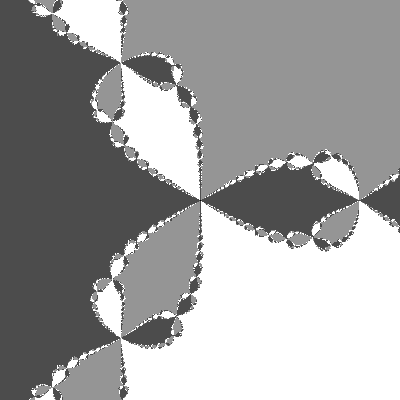
\includegraphics{fractale-z3+1-L.png}
\caption{Bassins d'attraction \(z \mapsto z^3+1\)}
\end{figure}

\begin{lstlisting}[language=Python]
\end{lstlisting}

\end{document}
